\documentclass[12pt]{article}
\usepackage[margin=1in]{geometry} 
\usepackage{amsmath,amsthm,amssymb,amsfonts}
\usepackage{tabto}
\usepackage{hyperref}

% Spacers:
% BEGIN BLOCK------------------------------------------
% END BLOCK============================================


\usepackage{wrapfig}

\newcommand{\N}{\mathbb{N}}
\newcommand{\Z}{\mathbb{Z}}

% CUSTOM SETTINGS
% BEGIN BLOCK------------------------------------------
% For equation system alignment
\usepackage{systeme,mathtools}
% Usage:
%	\[
%	\sysdelim.\}\systeme{
%	3z +y = 10,
%	x + y +  z = 6,
%	3y - z = 13}


% For definitions
\newtheorem{defn}{Definition}[section]
\newtheorem{thrm}{Theorem}[section]

% For circled text
\usepackage{tikz}
\newcommand*\circled[1]{\tikz[baseline=(char.base)]{
            \node[shape=circle,draw,inner sep=0.8pt] (char) {#1};}}

\newenvironment{problem}[2][Problem]{\begin{trivlist}
\item[\hskip \labelsep {\bfseries #1}\hskip \labelsep {\bfseries #2.}]}{\end{trivlist}}
%If you want to title your bold things something different just make another thing exactly like this but replace "problem" with the name of the thing you want, like theorem or lemma or whatever
 
%used for matrix vertical line
\makeatletter
\renewcommand*\env@matrix[1][*\c@MaxMatrixCols c]{%
  \hskip -\arraycolsep
  \let\@ifnextchar\new@ifnextchar
  \array{#1}}
\makeatother 

% END BLOCK============================================

\newtheorem*{lemma}{Lemma} %added
\newtheorem*{result}{Result} %added
\newtheorem*{theorem}{Theorem} %added
\theoremstyle{definition}
\newtheorem*{solution}{Solution} %added
\theoremstyle{plain}

% HEADER
% BEGIN BLOCK------------------------------------------
\usepackage{fancyhdr}
 
\pagestyle{fancy}
\fancyhf{}
\lhead{Exam \#3}
\rhead{Bryan Greener}
\cfoot{\thepage}
% END BLOCK============================================

% TITLE
% BEGIN BLOCK------------------------------------------
\title{Bryan Greener}
\author{MATH 2300 CRN:15163}
\date{2018-04-13}
\begin{document}
\maketitle
% END BLOCK============================================

\TabPositions{4cm}

\begin{enumerate}
\item[2.]Suppose a matrix is given as
\[ M=\begin{bmatrix}[rr]1&2\\1&1\\\end{bmatrix} \]
and define a pair of sequences according to
\begin{center}
$A_1=1$, $B_1=1$, and $\begin{bmatrix}[r]A_{n+1}\\B_{n+1}\\\end{bmatrix}=M\begin{bmatrix}[r]A_n\\B_n\\\end{bmatrix}$, $(n\geq 1)$
\end{center}
(a) Determine the first 10 terms of each of these sequences. (b) Determine the limit $\lim_{n\rightarrow\infty}(A_n/B_n)$, and prove your result. (Hint: Diagonalize $M$).
\begin{enumerate}
\item
\[ \begin{bmatrix}[r]3\\2\\\end{bmatrix},\begin{bmatrix}[r]7\\5\\\end{bmatrix},\begin{bmatrix}[r]17\\12\\\end{bmatrix},\begin{bmatrix}[r]41\\29\\\end{bmatrix},\begin{bmatrix}[r]99\\70\\\end{bmatrix},\begin{bmatrix}[r]239\\169\\\end{bmatrix},\begin{bmatrix}[r]577\\408\\\end{bmatrix},\begin{bmatrix}[r]1393\\985\\\end{bmatrix},\begin{bmatrix}[r]3363\\2378\\\end{bmatrix},\begin{bmatrix}[r]8119\\5741\\\end{bmatrix} \]
These results were found by writing a python program as follows:
\begin{verbatim}
import numpy as np
M = np.array([[1,2],[1,1]])
R = np.array([[1],[1]])
for i in range(11):
    print(R)
    R = np.dot(M,R)
\end{verbatim}

\item Next we diagonalize $M$ and get $P=\begin{bmatrix}[rr]\sqrt{2}&-\sqrt{2}\\1&1\\\end{bmatrix}$, $D=\begin{bmatrix}[rr]1+\sqrt{2}&0\\0&1-\sqrt{2}\\\end{bmatrix}$, and $P^{-1}=\begin{bmatrix}[rr]\frac{1}{2\sqrt{2}}&\frac{1}{2}\\-\frac{1}{2\sqrt{2}}&\frac{1}{2}\\\end{bmatrix}$. So $M^n=PD^nP^{-1}$. Thus $\lim_{n\rightarrow\infty}M^n=\lim_{n\rightarrow\infty}PD^nP^{-1}=PBP^{-1}$ where $B=\begin{bmatrix}[rr]\infty &0\\0&0\\\end{bmatrix}$.
Thus $\lim_{n\rightarrow\infty}M^n = PBP^{-1}=\begin{bmatrix}[rr]\infty&\infty\\\infty&\infty\\\end{bmatrix}$.\\
Since every item in the limit of $M$ is infinity, then multiplying $M\begin{bmatrix}[r]A_n\\B_n\\\end{bmatrix}$ for $n\rightarrow\infty$ will result in $\begin{bmatrix}[r]\infty\\\infty\\\end{bmatrix}$.\\ 
\end{enumerate}

\item[3.]The owner of a rapidly expanding business finds that for the first five months of the year the sales are \$4.0, \$4.4, \$5.2, \$6.4, and \$8.0 (thousands). After plotting these figures, the owner speculates that they follow a quadratic function. Find the last-squares quadratic polynomial fit to these data and use it to project sales for the remaining seven months of the year.
	\begin{center}
	\begin{tabular}{c|l}
	Month&Sales\\
	\hline
	1&\$4,000.00\\
	2&\$4,400.00\\
	3&\$5,200.00\\
	4&\$6,400.00\\
	5&\$8,000.00\\
	6&\$10,000.00\\
	7&\$12,400.00\\
	8&\$15,200.00\\
	9&\$18,400.00\\
	10&\$22,000.00\\
	11&\$26,000.00\\
	12&\$30,400.00\\
	\end{tabular}
	\end{center}
	These results were found by using the R functions lm() and predict() as seen below:
	\begin{verbatim}
	m = c(1,2,3,4,5)
	s = c(4.0,4.4,5.2,6.4,8.0)
	msquare = m**2
	rm = c(6,7,8,9,10,11,12)
	rmsquare = rm**2
	predict(lm(s~m + msquare), data.frame(m=rm,msquare=rmsquare))
	\end{verbatim}
	I then used the results in the 'fit' column as the sales column for the remaining months.

\item[5.] Use iterative methods to find the largest eigenvalue of the matrix
\[ M = \begin{bmatrix}[rrr]6&-4&1\\-4&6&-1\\1&-1&11\\\end{bmatrix} \]
and give a basis for its eigenspace. (Search using the key words "iterative" and "largest eigenvalue".)
\begin{solution}
In order to find the largest eigenvalue iteratively, I used the following function in python:
\begin{verbatim}
u = []
v = []
u.append(np.array([[1],[1],[1]]))
maxeigen = 0
for i in range(10000):
    v.append(M.dot(u[i]))
    u1 = v[i]
    u.append(v[i]/np.max(v[i]))
    u2 = u[i+1]
    maxeigen = np.max(v[i])
print(maxeigen)
\end{verbatim}

Eigenvalues: 12, 9, 2\\
Basis for eigenspace:  
\[ \left\{ \begin{bmatrix}[r]1\\1\\0\\\end{bmatrix},\begin{bmatrix}[r]-1\\1\\1\\\end{bmatrix},\begin{bmatrix}[r]\frac{1}{2}\\-\frac{1}{2}\\1\\\end{bmatrix} \right\} \]
I order to find these values, I wrote a function in Python which utilizes the numpy and sympy libraries which contain helpful linear algebra functions. The code used is below:
\begin{verbatim}
import numpy as np
from sympy import *
M = np.matrix([[6,-4,1],[-4,6,-1],[1,-1,11]])
E = np.linalg.eigvals(M)
print([Matrix((np.identity(3)*round(e)) - M).nullspace() for e in E])
\end{verbatim}
np.matrix just takes input and turns it into a matrix. np.linalg.eigvals() returns the eigenvalues of an input matrix in a list. np.identity(n) takes in an integer 'n' and returns an identity matrix of size $n\times n$. I then Matrix().nullspace() returns the nullspace for an input matrix. This is all wrapped in python list comprehension which loops through each index in E to form a list of lists which contains the basis for our eigenspace.
\end{solution}

\item[7.] Demonstrate an example of the Cayley-Hamilton theorem with a $5 \times 5$ matrix.
\begin{solution}
Let $A=\begin{bmatrix}[rrrrr]1&1&1&1&1\\0&2&1&1&1\\0&0&3&1&1\\0&0&0&4&1\\0&0&0&0&5\\\end{bmatrix}$.
Note that matrix $A$ is triangular with diagonal elements 1,2,3,4, and 5, and so its characteristic polynomial is
\[ \Delta(t)=(1-t)(2-t)(3-t)(4-t)(5-t) \]
So by expanding we get
\begin{align*}
\Delta(t)&=(1-t)(2-t)(3-t)(4-t)(5-t)\\
&= -t^5 + 15 t^4 - 85 t^3 + 225 t^2 - 274 t + 120\\
&= -A^5+15A^4-85A^3+225A^2-274A+120I\\
&= \begin{bmatrix}[rrrrr]0&0&0&0&0\\0&0&0&0&0\\0&0&0&0&0\\0&0&0&0&0\\0&0&0&0&0\\\end{bmatrix}
\end{align*}
This result was verified using the following python code below:
\begin{verbatim}
import numpy as np
A=np.matrix([[1,1,1,1,1],[0,2,1,1,1],[0,0,3,1,1],[0,0,0,4,1],[0,0,0,0,5]])
I=np.matrix([[1,0,0,0,0],[0,1,0,0,0],[0,0,1,0,0],[0,0,0,1,0],[0,0,0,0,1]])
print(-A**5 + 
      np.multiply(15,A**4) -
      np.multiply(85,A**3) + 
      np.multiply(225, A**2) -
      np.multiply(274,A) +
      np.multiply(120,I))
\end{verbatim}
\end{solution}

\item[8.]Demonstrate 3 non-trivial examples of the Singular Value Decomposition.
	\begin{enumerate}
	\item Let $M = \begin{bmatrix}[rrr]-149&-50&-154\\537&180&546\\-27&-9&-25\\\end{bmatrix}$.\\
	The SVD of $M$ is $M=UDV^\prime$ where
	\begin{align*}
	U&=\begin{bmatrix}[rrr]
	-0.26906707 & -0.67982121 & 0.68223605\\
	0.96200923 & -0.15566953 & 0.22428829\\
	-0.04627257 & 0.71666597 & 0.69587983\\\end{bmatrix}\\
	D&=\begin{bmatrix}[rrr]
	817.759668 & 0 & 0\\
	0 & 2.47497449 & 0\\
	0 & 0 & 0.00296452308\\\end{bmatrix}\\
	V^\prime &= \begin{bmatrix}[rrr]
	0.68227785 & 0.22871202 & 0.6943974\\
 	-0.66714135 & -0.19371852 & 0.71930213\\
 	0.29903068 & -0.95402513 & 0.02041339\\\end{bmatrix}
 	\end{align*}
 	I Got this result by using a python library function from numpy called linalg.svd. Below are the results:
 	\begin{verbatim}
	arr = np.array([[-149,-50,-154],[537,180,546],[-27,-9,-25]])
	U,D,V = np.linalg.svd(arr, full_matrices=True)
 	\end{verbatim}
 	I then verified this result by performing the following operations:
 	\begin{verbatim}
	IN    print(np.allclose(arr, U * np.diag(D) * V))
	OUT   True
 	
	IN    print(np.round([np.dot(U[:,i-1].A1, U[:,i].A1) 
	          for i in range(1,len(U))]))
	OUT   [-0., -0.]
	
	IN    print(np.round([np.dot(V[:,i-1].A1, V[:,i].A1) 
	          for i in range(1,len(V))]))
	OUT   [-0., -0.]
	
	IN    print(np.round(np.sum((np.multiply(U,U)),0)))
	OUT   [[1.,1.,1.]]
	
	IN    print(np.round(np.sum((np.multiply(V,V)),0)))
	OUT   [[1.,1.,1.]]
	
	IN    print(np.allclose(U.T * U, np.identity(len(U))))
	OUT   True
	
	IN    print(np.allclose(V.T * V, np.identity(len(V))))
	OUT   True
 	\end{verbatim}
 	The first result here is testing the result of $M=UDV$. The remaining functions are verifying the orthogonal properties of U and V. Functions two and three are verifying that the dot products across columns is equal to zero. Four and five are verifying that the columns are unit vectors. Finally functions six and seven are verifying that multiplying each matrix by its transpose results in the identity matrix.
	\item Let $M=\begin{bmatrix}[rrr]0&1&1\\\sqrt{2}&2&0\\0&1&1\\\end{bmatrix}$. Performing the same operations as above gives the results
	\begin{align*}
	U&=\begin{bmatrix}[rrr]-0.40824829 & 0.57735027 & -0.70710678\\
	-0.81649658 & -0.57735027 & 0\\
	-0.40824829 & 0.57735027 & 0.70710678\\\end{bmatrix}\\
	D&=\begin{bmatrix}[rrr]
	2.82842712 & 0 & 0\\
	0 & 1.41421356 & 0\\
	0 & 0 & 2.37213427e-17\\\end{bmatrix}\\
	V&=\begin{bmatrix}[rrr]
	-4.08248290e-01 & -8.66025404e-01 & -2.88675135e-01\\
	-5.77350269e-01 & -4.89172797e-17 & 8.16496581e-01\\
	-7.07106781e-01 & 5.00000000e-01 & -5.00000000e-01\\\end{bmatrix}
	\end{align*}
	Just as before, these results were verified to be accurate with the same functions from the previous example.
	\item Let $M=\begin{bmatrix}[rrrr]2&3&4&5\\3&4&5&6\\4&5&6&7\\5&6&7&8\\\end{bmatrix}$. Once again, this matrix has been run through the same program and its results (listed below) verified.
	\begin{align*}
	U&=\begin{bmatrix}[rrrr]
	-0.34897316 & -0.76040629 & 0.54422665 & 0.06178472\\
	-0.44231612 & -0.32304249 & -0.77168715 & 0.32326297\\
	-0.53565907 & 0.1143213 & -0.08930566 & -0.8318801\\
	-0.62900202 & 0.5516851 &  0.31676616 & 0.44683241\\\end{bmatrix}\\
	D&=\begin{bmatrix}
	2.09544512e+01 & 0 & 0 & 0\\
	0 & 9.54451150e-01 & 0 & 0\\
	0 & 0 & 8.73806904e-16 & 0\\
	0 & 0 & 0 & 4.73983730e-17\\\end{bmatrix}\\
	V&=\begin{bmatrix}[rrrr]
	-0.34897316 & -0.44231612 & -0.53565907 & -0.62900202\\
	0.76040629 & 0.32304249 & -0.1143213  & -0.5516851\\
	0.5477173 & -0.72850169 & -0.18614853 & 0.36693292\\
	0.00239892 & -0.41144293 & 0.81568911 & -0.4066451\\\end{bmatrix}
	\end{align*}
	\end{enumerate}

\end{enumerate}
Finally I will describe in detail the inner workings of a Feed Forward Neural Network that I implemented in Python.\\
\pagebreak
\section*{Introduction}

A feed forward neural network is a program which used a series of matrices which are one-to-one with adjacent matrices in which an input is given to one matrix then passed in only one direction through each layer of the network. The last matrix in this series is the result.\linebreak
\begin{wrapfigure}{r}{0.5\textwidth}
	\centering
	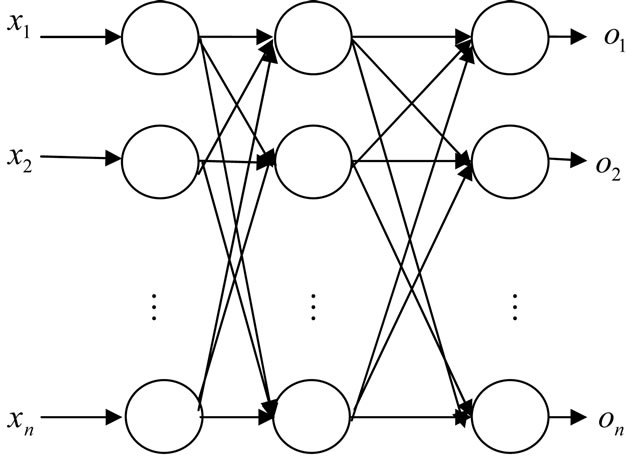
\includegraphics[width=0.35\textwidth]{FFNN.jpg}
\end{wrapfigure}

The graph to the right depicts a standard feed forward network with three layers and n nodes in each layer. The nodes in each layer can be viewed as being an $n\times 1$ matrix of values. At each node in each layer we store parameters for weight, activation, gradient, and bias. Weights at any layer refer to the value at each edge node between the current and previous layers. These values scale the output activation coming from the previous layer. Activations are the values at each node in a layer that are calculated by sending $z$ values through an activation function-- in this implementation we use a sigmoid function. The $z$ values at each layer are the result of the dot product of the activations of the previous layer and the edge weights between the previous and current layers. Each of these parameters will be described in greater detail later in this paper.\\

Feed forward neural networks are used in many applications of algorithm design and machine learning however this implementation is used to classify a $28\times 28$ image of a handwritten digit. The data set used for this network is the MNIST database of 70,000 images, 60,000 of which are used for training the network and the remaining 10,000 are used for testing. This separated set of training and testing images helps prevent over-fitting due to testing data also being used to train the network.\\

The specific implementation of FF Network used in this paper used backpropagation and mini-batch gradient descent which is calculated using the RMSprop and Nesterov Momentum algorithms. Each of these algorithms will be dissected and explained in detail relating to the linear algebra and calculus involved.

\section*{Forward Propagation}
Forward propagation as it relates to this implementation of a FF Network is the act of setting the activations and $z$ values of the input layer then updating each subsequent layer based on these inputs until the output layer matrix is returned. This output is the classification result of the network.\\

To start off, the weights and activations at each layer are set to random normalized values between -1.0 and 1.0. In order to calculate the $z$ values at any node, we take the dot product of the input activations and the edge weights between the previous and current layers. In this paper, we use $z_l$ and $W_l$ to refer to the activations and weights at any given layer. The only exception is that the input layer does not have any weights associated with it since it is the first layer in the network and therefore has no previous layer of which to connect.\\

This implementation also uses the sigmoid activation function to keep activation values between 0 and 1. At any layer, the activation of each node is calculated by the following equations
\begin{equation*}
z_l^n = \alpha_{l-1} \cdot W_l
\end{equation*}
\begin{equation*}
\alpha_l^n = \dfrac{1}{1 + e^{-z}}
\end{equation*}
where $l$ is the current layer and $n$ is a specific node at any layer. To simplify, the activation function will be denoted as $\alpha_l^n = \sigma(z_l)$. Thus the forward propagation result of a network with one input layer, two hidden layers, and one output layer can be depicted as follows
\begin{equation*}
\alpha_4^n = \sigma(z_3) \cdot W_3 = \sigma(z_2) \cdot W_2 = \sigma(z_1)
\end{equation*}
This guarantees an output at each node in the output layer which, for this implementation, will be a real value ranging from 0 to 9. However, this result will likely not be correct for the given input since the network has not yet been trained. Next the network needs to account for its mistakes and adjust to correct them.

\section*{Backward Propagation}
Backward Propagation, also referred to as "Backprop" is an algorithm which makes a backward pass through a neural network, updating the activations and weights as it moves back to the input layer. This is where the concept of cost and cost functions comes in to play.\\

The "cost" of an output node is the value relating to how far it is from the expected result in a training session. When training a network, the inputs and their expected results are known. So to calculate the cost at a node, an input is sent through the network in a forward pass. Then the activations at the output layer are used to calculate a cost, also known as a gradient, at each node. This is done using the following equations
\begin{equation*}
\sigma^\prime = \dfrac{e^{-z}}{(1+e^{-z})^2}
\end{equation*}
\begin{equation*}
E_l = \dfrac{\partial C}{\partial \alpha_l} = -(y - \alpha_l) \sigma^\prime(z_l)
\end{equation*}
This introduces a new function called sigmoid prime. This function is used in the calculation of the cost function at a given layer and is then used to calculate the partial derivative of the cost function in respect to the activation at the current layer. This partial derivative is also referred to as the error at the layer which will be denoted by a capital $E$. From here, this process cascades from the output layer to the input layer, hence the name \textit{back}propagation.\\

This method of sending errors backward through a network is what makes neural networks so powerful. It allows extremely complex algorithms to be run in polynomial times whereas with standard processing techniques they would be classified as NP-Hard. However there is still one step missing in this neural network. The term "gradient" was used but never explained. The next section breaks down this concept to help give a better understanding of what these costs and errors are actually used for.

\section*{Gradient Descent}
\begin{wrapfigure}{r}{0.50\textwidth}
	\centering
	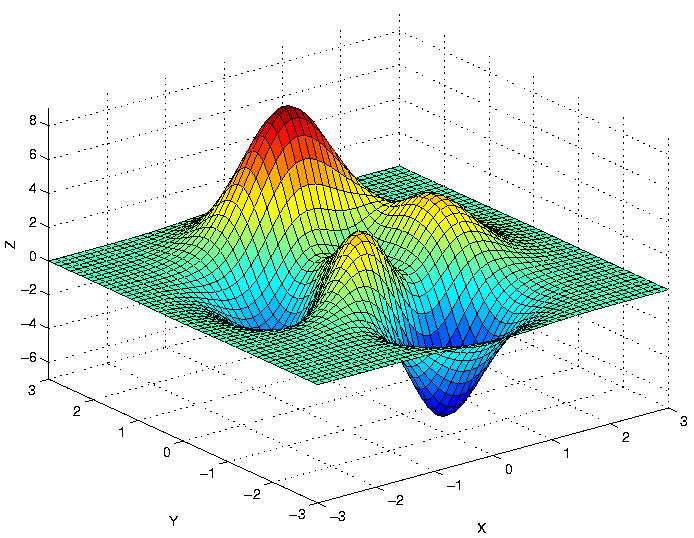
\includegraphics[width=0.50\textwidth]{Gradient.png}
\end{wrapfigure}

Pictured to the right is a graph that has no consistent shape. A simplified neural network can be depicted using this graph where the z-axis can be thought of as the cost of layers. The goal of the network is to minimize cost as the cost is the difference between the expected result and the observed result. Thus in order to do this, the network is looking for the minimum point in this graph. The problem with this is that it is far too complex of a graph to brute force by checking every single point in order to find a minimum. Thus the concept of a gradient descent function is the solution to this problem.\\

Gradient descent can be thought of as setting a ball at the top of one of the peaks of the graph then letting it roll down until it settles in place. As a concept, this is relatively simple. However implementing this takes a bit of effort. So the ball is at the top of a hill. The next step is to find the gradient at its current point then determine which way is down. This is done in the previous equations for calculating the cost and error. Next, the ball moves down the hill an amount proportional to the gradient. This is done to generalize the ball's movement so that it isn't always moving at a fixed rate which could result in overshooting the minimum or taking a very long time to reach a minimum.\\

This is the very basic concept of what a gradient descent algorithm is doing. It is just finding the local minimum point in a graph which will tell the network how much to adjust its weights and activations in order to result in the smallest error on a forward pass. In practice it is not quite as simple as this however as there are a few problems that come with gradient descent. Notice in the graph depicted earlier this section that there are two main valleys. The valley on the left is somewhat shallow which contains a local minimum for that region while the valley on the right is very deep and clearly contains the whole graph's minimum. This is where the network needs help from modified gradient descent algorithms like RMSprop and Nesterov Momentum.

\section*{RMSprop and Nesterov Momentum}
RMSprop (Root Mean Squared Propagation) and Nesterov Momentum are augmented Gradient Descent algorithms which aim to avoid problems that standard gradient descent algorithms such as Stochastic Gradient Descent have. With these standard methods, it is very likely that the ball rolling down the hill will land in a valley and think that it is in the graph's minimum just for it to be stuck in a local minimum whereas the graph's actual minimum is located elsewhere. Each algorithm has its own method of avoiding these issues to help improve performance and accuracy of the network.

\subsection*{RMSprop}
RMSprop resolves a performance issue caused by gradient descent where the ball rolling down the hill will zigzag due to subtle changes in gradient at any point in the graph which in turn causes the ball to reach its destination very slowly. RMSprop's solution to this problem is to keep track of previous gradients and average them in order to determine its next position. The following is an algorithm defining this behavior
\begin{align*}
r_t &= (1-\gamma)f^\prime(\delta_t)^2+\gamma r_{t-1}\\
v_{t+1} &= \dfrac{\eta}{\sqrt{r_t}}f^\prime (\delta_t)\\
\delta_{t+1}&= \delta_t-v_{t+1}
\end{align*}
\begin{center}\small Source: \url{http://climin.readthedocs.io/en/latest/rmsprop.html}\end{center}
This set of equations introduces a few new variables. $f^\prime(\delta)$ is the derivative of the $\delta$ calculated in previous sections in respect to the parameters at time step $t$. $\eta$ is a learn rate hyperparameter which is usually set to be between 0.0001 and 1.0. This variable is set based on trial and error during testing. $r$ is used as a cache for storing and averaging previous gradients. $\gamma$ is another hyperparameter which is usually set to 0.9, 0.99, or 0.999 and is set based on trial and error after testing. Finally $v$ stores individual gradients for each layer of the network.\\

\subsection*{Nesterov Momentum}
Nesterov Momentum helps to resolve the problem of the ball getting stuck in a local minimum with no way out. It does this by incorporating a pseudo-momentum that allows the ball to continue moving in its current trajectory when it reaches a local minimum. This is helpful because the continued movement can cause the ball to go over a peak past the local minimum and roll into the next local minimum. It does this using another new set of equations
\begin{align*}
v_t &= \gamma v_{t-1}+\eta\delta_\theta (\delta - \gamma v_{t+1})\\
\delta &= \delta - v_t
\end{align*}
Once again, $v$ is used as a cache of previous gradients in order to calculate how much pseudo-momentum the ball has as it is rolling.

\subsection*{RMSprop w/ Momentum}
The network in this paper incorporates both RMSprop and Nesterov Momentum to gain the benefits of each. This allows the ball to roll down the hill more efficiently and skip out of local minimums in search for the lowest point in the graph. The algorithm for this combination is as follows
\begin{align*}
\delta_{t+\frac{1}{2}} &= \delta_t-\beta v_t\\
r_t &=(1-\gamma) f^\prime(\delta_{t+\frac{1}{2}})^2 + \gamma r_{t-1}\\
v_{t+1} &= \beta v_t + \dfrac{\eta}{\sqrt{r_t}}f^\prime(\delta_{t+\frac{1}{2}})\\
\delta_{t+1} &= \delta_t - v_{t+1}
\end{align*}
\begin{center}\small{Source: \url{http://climin.readthedocs.io/en/latest/rmsprop.html}}\end{center}

The only new variables in this equation are $\delta_{t+\frac{1}{2}}$ which is just a temporary variable to store the half step of the new cost and $\beta$ which is another hyperparameter which through trial and error has been set to 5.0 as it produces the best results.\\

\section*{Conclusion}
Using each of the elements of this paper together, the neural network implementation was able to get a 50\% runtime improvement and a 4\% accuracy improvement over standard FF Networks using Stochastic Gradient Descent as their gradient descent algorithm. This brought the results to a 96\% classification accuracy when given 60,000 training images and testing against 10,000 testing images. Even more impressive however was a 25\% classification accuracy when given only 10 random training images and testing on 10,000 test images. This means that even given a very small set of sample information, the network was able to generalize the training results in order to correctly classify 2,500 images presented. At no point during testing is the network training further, the only operation performed is a forward pass after which the correct activations are accumulated.


\end{document}